\documentclass[tikz,border=10pt]{standalone}
\begin{document}
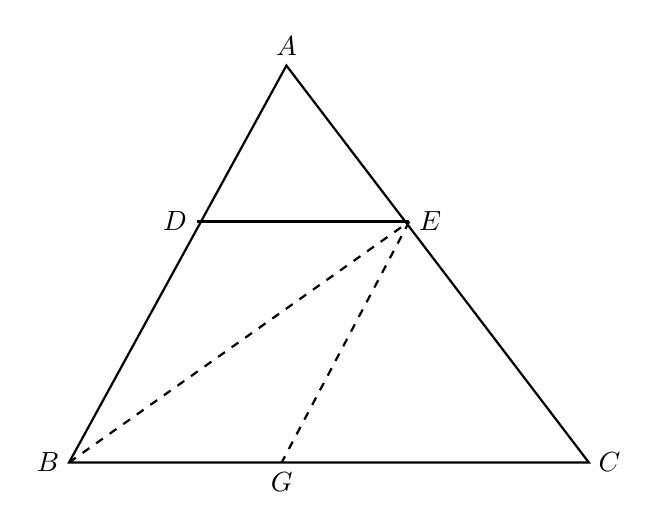
\begin{tikzpicture}[scale=1.2]
\coordinate (A) at (2.3,4.2);
\coordinate (B) at (0,0);
\coordinate (C) at (5.5,0);
\coordinate (D) at (1.35,2.55);
\coordinate (E) at (3.6,2.55);
\coordinate (G) at (2.25,0);

\draw[thick] (A) -- (B) -- (C) -- cycle;
\draw[thick] (D) -- (E);
\draw[dashed,thick] (B) -- (E);
\draw[dashed,thick] (E) -- (G);

\node[above] at (A) {$A$};
\node[left] at (B) {$B$};
\node[right] at (C) {$C$};
\node[left] at (D) {$D$};
\node[right] at (E) {$E$};
\node[below] at (G) {$G$};
\end{tikzpicture}
\end{document}
